\chapter{Entwicklung einer mobilen Anwendung}\label{mobile-app}
Auf Basis der ausgearbeiteten Ergebnisse aus Kapitel
\ref{chapter:motion-detection} soll nun eine mobile Anwendung entwickelt
werden. Ziel ist es die Ergebnisse mit einem praktischen Experiment für mobile
Plattformen zu verifizieren und damit die Forschungsfrage zu beantworten. Da
sich diese Arbeit vor allem mit dem Problem beschäftigen soll, wie eine
Bewegungserkennung auf mobilen Plattformen ausgeführt werden kann, soll eine
Android-App entwickelt werden, die Ergebnisse aus den vorherigen Kapiteln auf
einer mobilen Plattform getestet werden können. Android wird als Plattform
gewählt, da es zur Zeit die am häufigsten vertretene mobile Plattform ist und
ein entsprechendes Gerät leicht zur Verfügung steht. Zum Vergleich, Android
besitzt einen Marktanteil von 72,84\%, iOS einen von 26,34\% und 0,82\% werden
von sonstigen Plattformen
gehalten\footnote{https://www.statista.com/statistics/272698/global-market-share-held-by-mobile-operating-systems-since-2009/
  (besucht am 13.08.2021)}.

Die Anforderungen an die App sind recht simpel. Es sollen über die Kamera
Bewegungen identifiziert werden, wobei die erkannte Bewegungsart angezeigt
werden soll. Außerdem soll die Bewegungserkennung aus Kapitel \ref{chapter:motion-detection} in dieser App umgesetzt werden, sodass verschiedenste Bewegungen klassifiziert werden können.

\section{Implementierungsdetails}
Der Einfachheit halber werden zwei KNNs verwendet, um eine Bewegung zu
identifizieren. Das eine Netzwerk hat die Aufgabe, Schlüsselpunkte des
menschlichen Körpers in Bildern zu erkennen. Diese werden anschließend in einen
Puffer mit maximal 60 Elementen zwischengespeichert. Wird ein Element in den
Puffer hinzugefügt, so werden alle anderen Elemente zuerst um eine Position nach
hinten (rechts) verschoben. Der erste Slot ist nun dementsprechend leer und wird
von dem neuen Element belegt. Ist der Puffer bereits voll, so wird das letzte
Element entfernt. Ein Element dieses Puffers sind 17 Schlüsselpunkte des
menschlichen Körpers. Dieser Puffer bildet damit die Eingabe für das zweite
Netzwerk.  Dieses hat die Aufgabe, Schlüsselpunkte aus 60 Kamerabildern einer
Bewegungsklasse zuzuordnen.

Für die Schlüsselpunkterkennung wird MoveNets Lightning-Architektur
\cite{movenet} verwendet. Diese wurde speziell für mobile Geräte entwickelt,
sodass die Erkennung von Schlüs\-sel\-punk\-ten in Echtzeit durchgeführt werden
kann. Hier gilt es zu testen, ob die Performance in der Tat ausreichend ist, um
auf modernen, aber leistungsärmeren Geräten in Echtzeit zu laufen. Für die
Bewegungserkennung werden die verschiedenen Architekturen aus Kapitel
\ref{chapter:motion-detection} verwendet und getestet. Auch hier ist zu
überprüfen, ob diese in Zusammenarbeit mit MoveNet zu einer ausreichenden
Performance kommen. Eine ausreichende Performance wird dann angenommen, wenn
entsprechende Bewegungen über die Kamera bzw. über die entwickelte App richtig
erkannt wurden.

Für die Entwicklung der Android-App wurde \textit{Kotlin} verwendet. Zudem wird
die \textit{Ten\-sor\-Flow-Lite-API} (TFLite) verwendet, um die exportierten
Modelle auf Android auszuführen. Die in dieser Arbeit implementierten Modelle
wurden alle mit der \textit{TensorFlow-API} trainiert.  Da es sich dabei jedoch
um ein Desktop Framework handelt, wurden die trainierten Modelle im
\textit{Saved-Model}-Format gespeichert und anschließend in das TFLite-Format
umgewandelt. 

Es soll nun der allgemeine Aufbau der mobilen Anwendung besprochen werden. Im
ersten Schritt wurde sich Gedanken über mögliche Klassen der Anwendung gemacht.
Diese sind im UML-Klassendiagramm in Abbildung \ref{fig:uml-app} zu sehen. Als
Einstiegspunkt in dieser, sowie in jeder anderen Android-App, dient die
\texttt{MainActivity}-Klasse. Hier werden vor allem die View-Elemente der App
initialisiert. Auch die Modelle für das Erkennen von Bewegungen werden hier
geladen. Dies ist zum einen das MoveNet-Lightning-Modell\footnote{MoveNet-Lightning, https://tfhub.dev/google/movenet/singlepose/lightning/4} für die
Schlüsselpunkterkennung und zum anderen das MotionNet aus Kapitel
\ref{chapter:motion-detection}. Warum die beiden Modelle nicht in ein einziges
Modell zusammengefügt worden sind, hat den Grund, dass die Schlüsselpunkte in
den dazugehörigen Puffer gespeichert werden sollen. Dieser wird dann
anschließend vom MotionNet ausgelesen und interpretiert, sodass eine
Bewegungserkennung stattfinden kann. Die Ausgabe von einem
Schlüsselpunktdetektor kann demnach nicht direkt als Eingabe für das MotionNet
dienen. Dies liegt natürlich auch daran, dass versucht wird, eine Bewegung in
Echtzeit zu erkennen. Deshalb ist es notwendig, dass die Bilder der Kamera auch
in Echtzeit analysiert werden. Erst wenn diese Abtastung ein bestimmtes
Zeitfenster beinhaltet, kann eine zeitabhängige Änderung einer Pose erkannt
werden. Die beiden geladenen Modelle werden nun in eine dafür vorgesehene Klasse
verwaltet. \texttt{MotionDetector} soll die Erkennungslogik implementieren, was
unter anderem die Implementierung des Schlüsselpunktpuffers (siehe Abbildung
\ref{fig:camera-frame-buffer}) bedeutet. Diese Klasse wird abstrakt umgesetzt,
damit neue Modelle zum Erkennen von Bewegungen einfach von ihr erben und
entsprechende Methoden überschreiben können, um den Weg in die Anwendung
leichter finden zu können. Als Beispiel hierfür wurde das \texttt{MotionNet}
implementiert, welches nun von der abstrakten Klasse erbt. Hier werden die
Modelle als \textit{Interpreter} der \textit{TensorFlow-Lite-API} verwaltet. Die
Inferenz der Modelle wird schließlich in den zu überschreibenden Methoden
ausgeführt. Damit die Ausführung der Modelle überhaupt stattfinden kann, müssen
Bilder über die Kamera in die Anwendung geleitet werden. Dies wird mithilfe der
implementierten \texttt{CameraManager}-Klasse umgesetzt. Diese stellt das
aktuelle Bild der Kamera über ein dafür vorgesehenes Steuerelement dar und
bietet eine Schnittstelle zum Abfangen einzelner Frames. Diese Frames werden
anschließend über die \texttt{MainActivity} in die Bewegungserkennung geleitet.
Nach der Inferenz wird das User-Interface mithilfe der \texttt{MainActivity}
aktualisiert und die Ergebnisse dargestellt. Speziell für die Darstellung der
Schlüsselpunkte und der Bewegungsart wird die View-Klasse \texttt{PersonOverlay}
umgesetzt. Diese stellt alle aus der Bewegungserkennung resultierenden
Ergebnisse grafisch dar.

\begin{figure}
    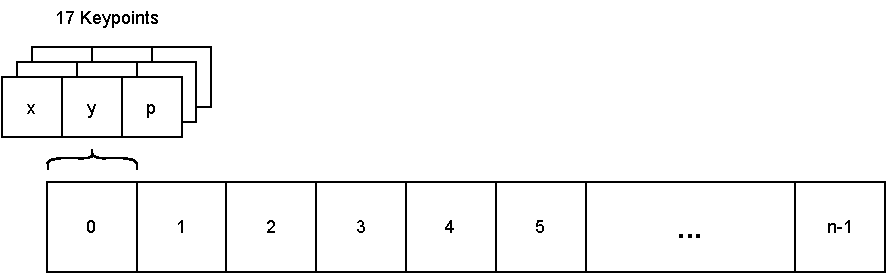
\includegraphics[width=\textwidth]{images/camera_frame_buffer.pdf}
    \caption{Schematische Darstellung des Puffers der Bewegungserkennung,
    welcher $n = 60$ Schlüsselpunkte des menschlichen Körpers speichert.}
    \label{fig:camera-frame-buffer}
\end{figure}

\begin{figure}
    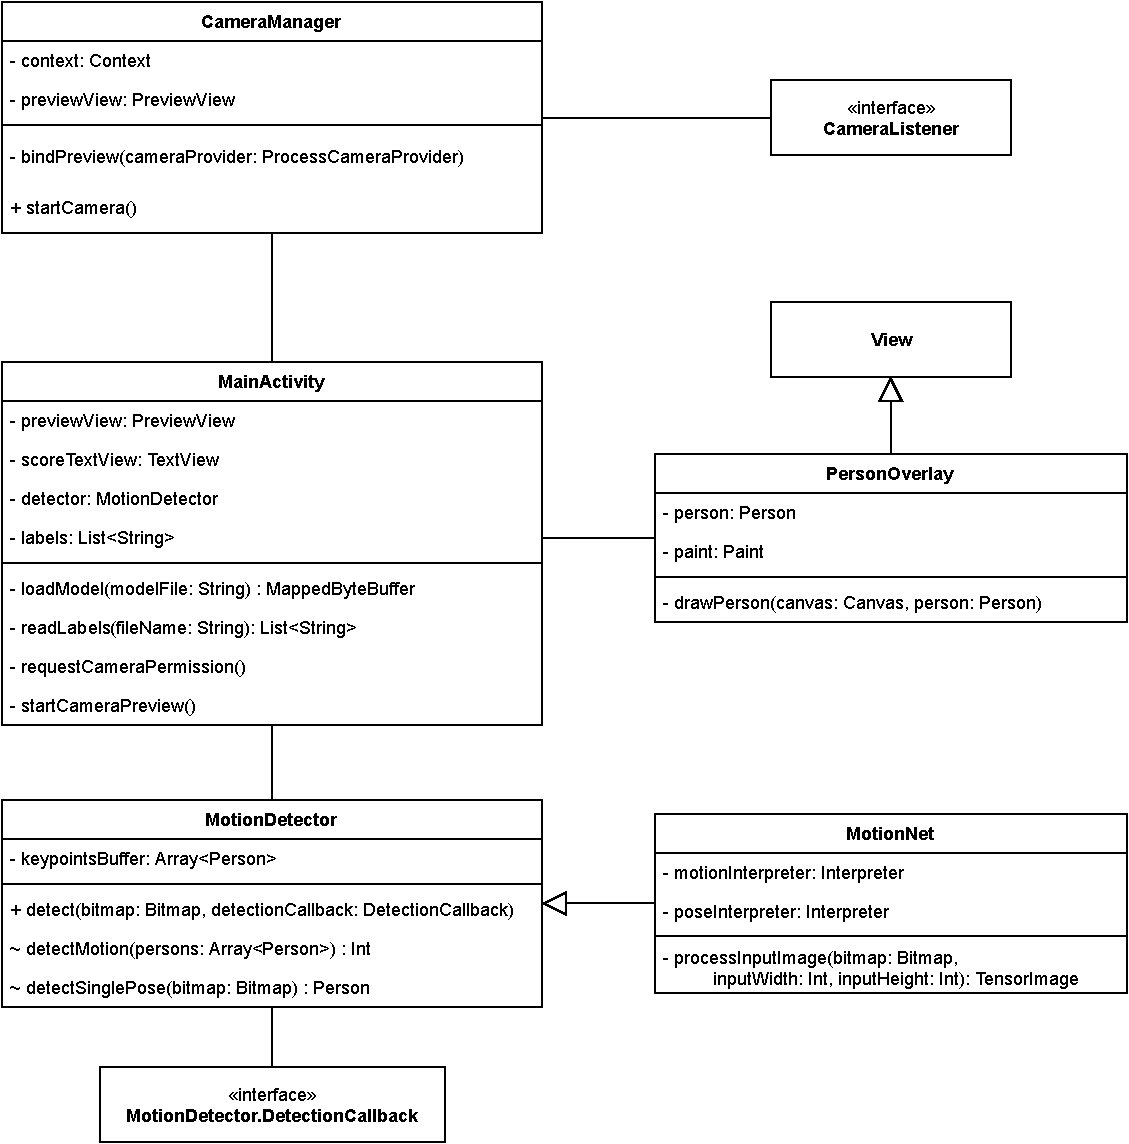
\includegraphics[width=\textwidth]{images/app_uml.pdf}
    \caption{UML-Klassendiagramm der mobilen Anwendung zum Testen der
    Machine-Learning-Modelle für die Bewegungserkennung.}
    \label{fig:uml-app}
\end{figure}

\section{Testaufbau und Ergebnisse}
Die Bewegungserkennung aus den vorherigen Abschnitten soll nun mithilfe der
implementierten mobilen Applikation in der Praxis getestet werden. Hierfür muss
vorerst der Testaufbau besprochen werden, sodass die Ergebnisse nachvollziehbar
und reproduzierbar sind. Als Plattform wird Android zusammen mit ausgewählten
mobilen Geräten verwendet. Ziel ist es herauszufinden, ob die Bewegungserkennung
auf moderner, aber auch auf älterer Hardware in Echtzeit ausführbar ist. Tabelle
\ref{table:android-tests} zeigt die durchgeführten Testläufe und deren
Ergebnisse. Besonders hervorzuheben ist die Ausführungsgeschwindigkeit auf
älteren Geräten. So konnte die Bewegungserkennung mit bis zu 6 FPS auf einem
Samsung Galaxy S6 Edge ausgeführt werden. Als Testdaten wurden echte Personen
mit echten Bewegungen mit einem Abstand von 2 Meter abgefilmt. Da es sich
hierbei um eine Echtzeiterkennung handelt und deshalb die Umgebungsbedingungen
durch beispielsweise Kamerawackeln, Lichteinflüssen und Rauschen nicht immer
exakt equivalent sind, muss die Messung der Erkennungsgenauigkeit etwas genauer
erläutert werden.

Beim Testen der Bewegungserkennung wurde sich die Frage gestellt, wie lange
eine Bewegung ausgeführt werden muss, um den Puffer komplett mit dieser
Bewegung zu füllen, ohne dass andere Bewegungsarten in diesem enthalten sind.
Hierfür wird nach dem Beginn einer neuen Bewegung eine Vorlaufzeit festgelegt,
die sicher stellt, dass nach Ablauf dieser Zeit der komplette Puffer mit einer
Bewegung gefüllt ist. Je größer der Puffer ist, desto größer ist auch die
Vorlaufzeit. Gleichzeitig verringert sich die benötigte Vorlaufzeit, je
schneller die Bewegungserkennung ausgeführt werden kann. Das bedeutet
lediglich, dass eine schnellere Posenerkennung den Puffer schneller füllt.
Mathematisch zusammengefasst verhält sich die Vorlaufzeit $t$ proportional zur
Puffergröße $n_\mathrm{buffer}$ und der Inferenzzeit $t_\mathrm{inference}$ der
Bewegungserkennung.

\begin{equation}\label{eq:preruntime}
  t = n_\mathrm{buffer} \cdot t_\mathrm{inference}
\end{equation}

\begin{table}
    \footnotesize
    \begin{tabularx}{\textwidth}{l|l|X|l|l|l|l}
        \hline
        Mobile Device & CPU & Inference Time (ms) & FPS & $n_\mathrm{buffer}$ & $t$ & Accuracy \\ \hline

        \multirow{3}{*}{Samsung Galaxy S6 Edge} & \multirow{3}{*}{Exynos 7 Octa 720} & \multirow{3}{*}{160} & \multirow{3}{*}{6} & 10 & 1.67 & $2 / 3$ \\ \cline{5-7}
        & & & & 20 & 3.33 & $3 / 3$ \\ \cline{5-7}
        & & & & 60 & 10 & $1 / 3$ \\ \hline

        \multirow{3}{*}{Samsung Galaxy S10} & \multirow{3}{*}{Exynos 9820} & \multirow{3}{*}{71} & \multirow{3}{*}{14} & 10 & 0.71 & $3/3$  \\ \cline{5-7}
        & & & & 20 & 1.43 & $3/3$ \\ \cline{5-7}
        & & & & 60 & 4.26 & $1/3$ \\ \hline
    \end{tabularx}
    \caption{Testergebnisse der Bewegungserkennung auf verschiedenen mobilen Geräten. Die Genauigkeit gibt an, wie viele Bewegungen im Testszenario richtig erkannt wurden. Getestete Bewegungen waren Liegestütze, Klimmzüge und Bankdrückübungen.}
    \label{table:android-tests}
\end{table}

Der Tabelle \ref{table:android-tests} kann man entnehmen, dass drei festgelegte
Puffergrößen auf unterschiedlich schnellen Geräten ausgeführt wurden. Anhand
der Gleichung \ref{eq:preruntime} wurden die entsprechenden Vorlaufzeiten
$t$ berechnet. Während des Testens wurde eine Bewegung für 10 Sekunden plus die
Vorlaufzeit ausgeführt. Zu Erkennen ist, dass ein größerer Puffer nicht
bedeutet, dass eine bessere Erkennungsrate erzielt wird. Zusätzlich bedeutet
ein größerer Puffer auch, dass die Vorlaufzeit entsprechend länger sein muss.
Dies kann dazu führen, dass keine Echtzeiterkennung möglich ist, da die
Vorlaufzeit $t$ einfach zu groß ist. Unter dem Samsung Galaxy S6 Edge+ wurden
die besten Erkennungsraten mit einem Puffer mit 20 Elementen erreicht. Es
wurden alle Bewegungen korrekt erkannt bei einer Vorlaufzeit von 3.33 Sekunden.
Auf dem Samsung Galaxy S10 haben Puffer mit einer Größe von 10 oder 20 zu den
besten Ergebnissen geführt. Da dieses Gerät eine stärkere Hardware besitzt,
sind die Vorlaufzeiten entsprechend geringer als die bei dem S6 Edge+. Hier
kann sogar mit einem Puffer mit nur 10 Elementen verwendet werden, was die
Vorlaufzeit auf 0.71 Sekunden reduziert bei gleicher Erkennrate. Dies bedeutet
lediglich, dass eine Erkennung um 0.71 Sekunden verzögert stattfindet. In dem
Praxistest wurde außerdem festgestellt, dass eine Erkennung einer wechselnden
Bewegung sogar vor der Vorlaufzeit möglich ist.  Insgesamt wurde die
Bewegungserkennung auf beiden Geräten in Echtzeit mit einer hohen Genauigkeit
ausgeführt.
